% -*- TeX -*-
%
% ----------------------------------------------------------------------
%
%                           Brad T. Aagaard
%                        U.S. Geological Survey
%
% {LicenseText}
%
% ----------------------------------------------------------------------
%
\documentclass[pdftex,cig,slideColor]{pp4slides}
\usepackage{amsmath}
\usepackage{array}
\usepackage{xspace}
\usepackage{multirow}
\usepackage{ulem}

\newcommand{\newfeature}[1]{{\color{blue}#1}}

\renewcommand{\movielink}[2]{\href{run:#1.avi}{#2}}

\title{PyLith 1.5\\
  Friction, Small Strains, and Elastoplasticity}
\author{Brad Aagaard and Charles Williams\\[10pt]
  Matthew Knepley and Surendra Somala}
\institution{\includegraphics[height=2cm]{../../logos/cig}}
\date{June 15, 2010}

% --------------------------------------------------------- DOCUMENT
\begin{document}

% ------------------------------------------------------------ SLIDE
\maketitle

% ------------------------------------------------------------ SLIDE
\foilhead{Outline}
  \summary{Major new features in PyLith 1.5 and important issues}

  \begin{itemize}
  \item Insertion of cohesive cells and fault edges
  \item Dynamic fault ruptures (frictional interfaces)
    \begin{itemize}
    \item Implementation
    \item Fault constitutive models
      \begin{itemize}
      \item Static friction
      \item Linear slip-weakening
      \item Rate and state friction w/ageing law
      \end{itemize}
    \end{itemize}
  \item Drucker-Prager elastoplastic bulk rheology
  \end{itemize}


\bgadd{\vspace*{7.9in}%
  \begin{center}%
    \includegraphics[height=14mm]{../../logos/cig}
  \end{center}}


% ------------------------------------------------------------ SLIDE
\foilhead{Insertion of Cohesive Cells}
  \summary{Topology of fault edge is ambiguous}


  \vfill
  {\bf Constrain slip to be zero at fault edge to remove ambiguity in
  behavior.}
 \vfill
  \begin{center}
    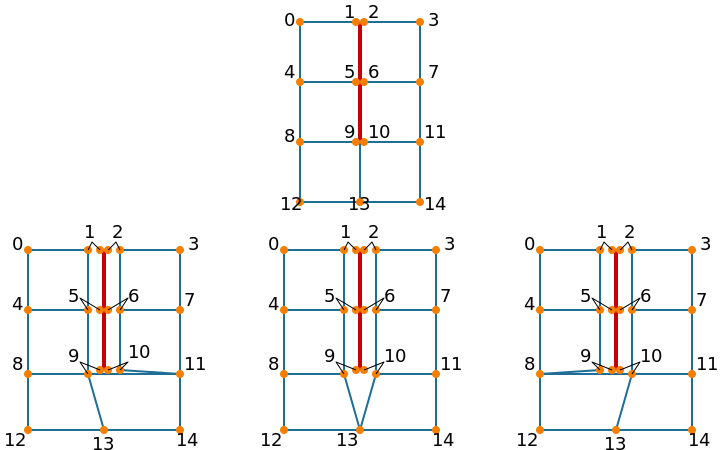
\includegraphics{figs/fault_edge}
  \end{center}
  \vfill


% ------------------------------------------------------------ SLIDE
\foilhead{Dynamic Fault Ruptures}
  \summary{Frictional interface with fault constitutive model}

  \vfill
  \vspace*{-14pt}
  \begin{equation}
    \left( \begin{array}{cc}
        A & C^T \\ C & 0
      \end{array} \right)
    \left( \begin{array}{c}
        u \\ l
      \end{array} \right)
    =
    \left( \begin{array}{c}
        b \\ d
      \end{array} \right)
  \end{equation}
  \vfill

  Nonlinear solve:
  \begin{itemize}
  \item Begin each iteration usng current estimates of slip and fault
    tractions (Lagrange multipliers)
  \item Iteration algorithm
    \begin{enumerate}
    \item Compute allowable fault traction using fault constitutive
      model
    \item If fault tractions (Lagrange multipliers) do not exceed values
      allowed by friction
     \begin{enumerate}
      \item No change to Lagrange multipliers
      \item Current estimate of slip is correct
      \end{enumerate}
    \item If fault tractions (Lagrange multipliers) exceed  values
      allowed by friction
     \begin{enumerate}
      \item Reduce Lagrange multipliers to be compatible with friction
      \item Update slip estimate based on change in Lagrange multipliers
      \end{enumerate}
    \end{enumerate}
  \end{itemize}
  
% ------------------------------------------------------------ SLIDE
\foilhead{Dynamic Fault Ruptures: Frictional Interfaces}
  \summary{Updating slip according to friction}

  \vfill
  Equations for conventional DOF:
  \vspace*{-14pt}
  \begin{equation}
    \underline{A} \vec{u} + \underline{C}^T \vec{l} = \vec{b}
  \end{equation}
  Variation in displacement field for variation in Lagrange multiplier
  values:
  \vspace*{-14pt}
  \begin{equation}
    \underline{A} \partial\vec{u} = -\underline{C}^T \partial\vec{l}
  \end{equation}
  Solve for $\partial \vec{u}$ using portion of A associated
  w/fault DOF \\
  Example PETSc setting for friction solve: {\tt friction\_pc\_type = asm}
  \begin{itemize}
  \item Slip estimate is exact if all other DOF are fixed.
  \item Slip estimate is good approx. (fast convergence) if
    deformation for fault slip decays rapidly w/distance from fault
  \item Slip estimate is poor approx. (slow convergence) if
    deformation for fault slip is nearly uniform (see examples)
  \end{itemize}
  
 
% ------------------------------------------------------------ SLIDE
\foilhead{Dynamic Fault Ruptures: Frictional Interfaces}
  \summary{}

  \begin{itemize}
  \item Tractions driving slip, superposition of
    \begin{itemize}
    \item Constant initial values imposed directly on the fault surface
    \item Computed from deformation
    \end{itemize}
  \item Must use nonlinear solver with sparse system Jacobian matrix
  \item Parameters
    \begin{description}
    \item[db\_initial\_tractions] Spatial database with initial tractions
    \item[friction] Fault constitutive model
    \end{description}
  \end{itemize}
  

% ------------------------------------------------------------ SLIDE
\foilhead{Fault Constitutive Models}
  %\summary{}

  \vfill
  \begin{equation}
    T_f = \begin{cases}
      T_c - \mu_f T_n & T_n \leq 0 \\
      0 & T_n > 0
    \end{cases}
  \end{equation}
  \vfill

  \begin{itemize}
  \item Static friction
    \begin{equation}
    \vspace*{-14pt}
      \mu_f = \mu_s
    \end{equation}
  \item Linear slip-weakening friction
    \vspace*{-14pt}
    \begin{equation}
      \mu_f = \begin{cases}
        \mu_s - \frac{d(t)}{d_0}(\mu_s - \mu_d) & d(t) \leq d_0 \\
        \mu_d & d(t) > d_0
      \end{cases}
    \end{equation}
  \item Rate and state friction
    \vspace*{-14pt}
    \begin{gather}
      \mu_f = \mu_s + a \ln \left(\frac{V}{V_0} \right) + b \ln \left( \frac{V_0
        \theta}{L} \right) \\
      \frac{d\theta}{dt} = 1 - \frac{V \theta}{L}
    \end{gather}
 \end{itemize}


% ------------------------------------------------------------ SLIDE
\foilhead{Fault Constitutive Model: Parameters}
  \summary{Analogous to bulk constitutive model}

  \begin{description}
  \item[db\_properties] Spatial database with fault constitutive model parameters
  \item[db\_initial\_state] Spatial database with initial state variables
  \end{description}

% ------------------------------------------------------------ SLIDE
\foilhead{Dynamic Fault Ruptures Example}
  \summary{{\tt examples/3d/hex8 step14.cfg}}

\movie{0.5in}{0.0in}{8.0in}{5.7778in}{movies/step14}%
 

% ------------------------------------------------------------ SLIDE
\foilhead{Small Strains}
  \summary{Total Lagrangian formulation}

  \begin{itemize}
  \item Common applications
    \begin{itemize}
    \item No strain for rigid body motion
    \item Overburden pressure increases when cross-section decreases
    \end{itemize}
  \item Stress/strain tensors
    \begin{description}
    \item[Strain metric] Green-Lagrange strain tensor
      \vspace*{-14pt}
      \begin{equation}
        \varepsilon_{ij} = \frac{1}{2}(u_{i,j} + u_{j,i} + u_{k,i}u_{k,j})
      \end{equation}
    \item[Stress metric] Second Piola-Kirchhoff stress tensor
      \vspace*{-14pt}
      \begin{equation}
        S_{ij} = C_{ijkl} \varepsilon_{kl}
      \end{equation}
    \end{description}
  \item Nonlinear solver selected automatrically when using sparse
    system Jacobian matrix
  \end{itemize}

% ------------------------------------------------------------ SLIDE
\foilhead{Drucker-Prager Elastoplastic Bulk Rheology}
  \summary{Smooth approximation to Mohr-Coulomb yield criterion}

  \begin{itemize}
  \item Yield surface forms a smooth cone in principal stress space
    that is coincident with the outer apices of the Mohr-Coulomb yield
    envelope.
  \item Non-associated plastic flow (different yield and flow
    functions), which allows control over the unrealistically large
    amounts of dilatation that are sometimes predicted by the
    associated model.
  \item Perfectly plastic implementation, does not include hardening
 \item {\bf Must use nonlinear solver with sparse system Jacobian matrix}
  \end{itemize}
  
% ------------------------------------------------------------ SLIDE
\foilhead{Drucker-Prager Elastoplastic Bulk Rheology}
  \summary{Smooth approximation to Mohr-Coulomb yield criterion}

  \vfill
  \begin{center}
    \includegraphics[scale=0.88]{figs/DruckerPragerYieldSurf2D}
    \includegraphics[scale=0.88]{figs/DruckerPragerYieldSurf3D}
  \end{center}
  \vfill


% ------------------------------------------------------------ SLIDE
\foilhead{Drucker-Prager Elastoplastic Bulk Rheology}
  %\summary{Constitutive Model}

  \vfill
  \begin{itemize}
  \item Yield function
    \vspace*{-14pt}
    \begin{gather}
      f (\underline{\sigma}) = \alpha_{f} I_{1} + \sqrt{J_{2}^{\prime}}-\beta, \\
      \alpha_{f } =\frac{2\sin\phi}{\sqrt{3}\left(3-\sin\phi\right)} \\
      \beta=\frac{6c\cos\phi}{\sqrt{3}\left(3-\sin\phi\right)}
    \end{gather}
    \vspace*{-36pt}
  \item Flow function
    \vspace*{-14pt}
    \begin{gather}    
      g\left(\underline{\sigma}\right) = \alpha_{g}I_{1}+\sqrt{J_{2}^{\prime}} \\
      \alpha_{g}=\frac{2\sin\psi}{\sqrt{3}\left(3-\sin\psi\right)}
    \end{gather}
    \vspace*{-36pt}
  \end{itemize}
  \vfill
  {\small
    \begin{description}
    \item First stress invariant: $\; I_{1}=\sigma_{ii}$
    \item Second deviatoric stress invariant:
      $J_{2}^{\prime}=\frac{1}{2}\sigma_{ij}\sigma_{ij}$
    \item Friction angle: $\phi$
    \item Cohesion: $c$
    \item Dilatation angle: $\psi$
    \end{description}
  }

 
% ======================================================================
\end{document}


% End of file
